% =============================================================================
%
%  ██████╗  ██████╗███╗   ███╗    ██████╗    ██████╗ 
%  ██╔══██╗██╔════╝████╗ ████║    ╚════██╗  ██╔═████╗
%  ██████╔╝██║     ██╔████╔██║     █████╔╝  ██║██╔██║
%  ██╔══██╗██║     ██║╚██╔╝██║    ██╔═══╝   ████╔╝██║
%  ██████╔╝╚██████╗██║ ╚═╝ ██║    ███████╗  ╚██████╔╝
%  ╚═════╝  ╚═════╝╚═╝     ╚═╝    ╚══════╝   ╚═════╝ 
%
%  MASTER DOCUMENTATION FRAMEWORK
%  ==============================
%  
%  Das integrierte Meta-Framework für EBF
%  
%  Von der Idee zum fertigen Dokument in 5 Schritten
%
% =============================================================================

\documentclass[12pt,a4paper]{article}
\usepackage[margin=2cm]{geometry}
\usepackage{amsmath,amssymb}
\usepackage{booktabs}
\usepackage{colortbl}
\usepackage{longtable}
\usepackage{tcolorbox}
\usepackage{enumitem}
\usepackage{hyperref}
\usepackage{xcolor}
\usepackage{array}
\usepackage{tikz}
\usetikzlibrary{shapes,arrows,positioning}

\tcbuselibrary{skins,breakable}

% Custom colors
\definecolor{bcmblue}{RGB}{0,82,147}
\definecolor{bcmgreen}{RGB}{0,128,0}
\definecolor{bcmred}{RGB}{180,0,0}
\definecolor{bcmyellow}{RGB}{255,193,7}
\definecolor{bcmpurple}{RGB}{128,0,128}

\title{\Huge\textbf{EBF Master Documentation Framework}\\[1em]
\Large Von der Idee zum fertigen Dokument\\[0.5em]
\normalsize Version 1.0 -- Januar 2026}
\author{BEATRIX Research Group\\FehrAdvice \& Partners AG}
\date{}

\begin{document}
\maketitle

\begin{tcolorbox}[colback=bcmblue!10!white, colframe=bcmblue, 
    title=\textbf{Zweck dieses Frameworks}]
    
Dieses Master-Framework integriert alle Meta-Ebenen der EBF Dokumentation:

\begin{enumerate}[nosep]
\item \textbf{SPEZIFIKATION:} Die 12 Dimensionen jedes Dokuments
\item \textbf{FORMAT:} Automatische Ableitung des Dokumenttyps
\item \textbf{ARCHITEKTUR:} Einordnung in Haupt vs. Appendix
\item \textbf{SCOPE:} Umfang und Tiefe bestimmen
\item \textbf{STRUKTUR:} Template und Gliederung ableiten
\end{enumerate}

\textbf{Ergebnis:} Für jedes Thema sofort wissen WO, WIE VIEL, und WIE es dokumentiert wird.

\end{tcolorbox}

\tableofcontents
\newpage

% #############################################################################
%
%                    TEIL I: DAS GESAMTSYSTEM
%
% #############################################################################

\part{Das Gesamtsystem}

% =============================================================================
\section{EBF Dokumenten-Architektur}
% =============================================================================

\subsection{Die Zwei-Ebenen-Struktur}

\begin{center}
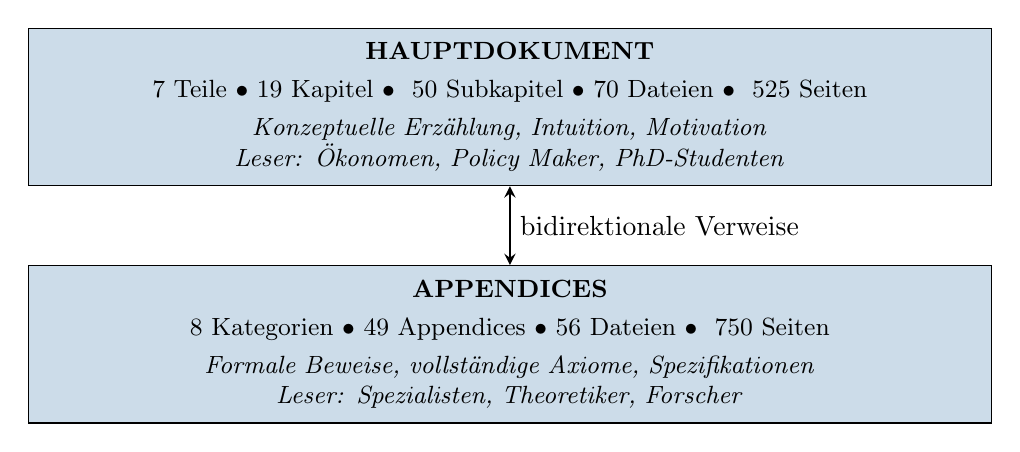
\begin{tikzpicture}[node distance=2cm, auto,
    box/.style={rectangle, draw, fill=bcmblue!20, text width=12cm, 
                text centered, minimum height=2cm, font=\small},
    arrow/.style={thick,->,>=stealth}]
    
\node[box] (main) {
    \textbf{HAUPTDOKUMENT}\\[0.3em]
    7 Teile $\bullet$ 19 Kapitel $\bullet$ ~50 Subkapitel $\bullet$ 70 Dateien $\bullet$ ~525 Seiten\\[0.3em]
    \textit{Konzeptuelle Erzählung, Intuition, Motivation}\\
    \textit{Leser: Ökonomen, Policy Maker, PhD-Studenten}
};

\node[box, below=1cm of main] (app) {
    \textbf{APPENDICES}\\[0.3em]
    8 Kategorien $\bullet$ 49 Appendices $\bullet$ 56 Dateien $\bullet$ ~750 Seiten\\[0.3em]
    \textit{Formale Beweise, vollständige Axiome, Spezifikationen}\\
    \textit{Leser: Spezialisten, Theoretiker, Forscher}
};

\draw[arrow, <->] (main) -- node[right] {bidirektionale Verweise} (app);

\end{tikzpicture}
\end{center}

\subsection{Die 4 fundamentalen Fragen}

Jeder Inhalt in EBF adressiert mindestens eine dieser Fragen:

\begin{table}[htbp]
\centering
\renewcommand{\arraystretch}{1.5}
\begin{tabular}{@{}cllll@{}}
\toprule
\textbf{Code} & \textbf{Frage} & \textbf{Antwort} & \textbf{Symbol} & \textbf{CORE Appendix} \\
\midrule
\cellcolor{bcmblue!20}\textbf{WHO} & Wer hat Utility? & Aggregationsebenen & $L \in \{0,...,\infty\}$ & AAA \\
\cellcolor{bcmgreen!20}\textbf{WHAT} & Was ist Utility? & FEPSDE-Dimensionen & $d \in \{F,E,P,S,D,E\}$ & C \\
\cellcolor{bcmyellow!20}\textbf{HOW} & Wie interagieren sie? & Complementarity & $\gamma_{ij}$ & B \\
\cellcolor{bcmpurple!20}\textbf{WHEN} & Wann wirkt Kontext? & Ψ-Dimensionen & $\Psi = (\Psi_1,...,\Psi_8)$ & V \\
\bottomrule
\end{tabular}
\end{table}

\subsection{Die 8 Appendix-Kategorien}

\begin{table}[htbp]
\centering
\renewcommand{\arraystretch}{1.3}
\small
\begin{tabular}{@{}clccp{5cm}@{}}
\toprule
\textbf{Kat.} & \textbf{Name} & \textbf{Anzahl} & \textbf{Scope} & \textbf{Zweck} \\
\midrule
\cellcolor{bcmred!20}CORE & Fundamentaltheorie & 4 & A4--A5 & Beantwortet WHO/WHAT/HOW/WHEN \\
FORMAL & Mathematik & 4 & A2--A5 & Formale Ableitungen, Beweise \\
DOMAIN & Anwendung & 13 & A3 & Feldspezifische Anwendung \\
CONTEXT & Ψ-Framework & 3 & A3--A4 & Zeit/Raum/Kontext \\
METHOD & Methodik & 4 & A2--A3 & Empirische Methoden \\
PREDICT & Vorhersagen & 7 & A3 & Testbare Predictions \\
LIT & Literatur & 10 & A2--A3 & Autor/Themen-Integration \\
REF & Nachschlagen & 4 & A2--A3 & Glossar, Beispiele \\
\bottomrule
\end{tabular}
\end{table}


% #############################################################################
%
%                    TEIL II: DER 5-SCHRITTE-PROZESS
%
% #############################################################################

\part{Der 5-Schritte-Prozess}

\begin{tcolorbox}[colback=bcmgreen!10!white, colframe=bcmgreen, 
    title=\textbf{Von der Idee zum Dokument in 5 Schritten}]

\begin{center}
\Large
\textbf{IDEE} $\xrightarrow{\text{Schritt 1}}$ 
\textbf{SPEC} $\xrightarrow{\text{Schritt 2}}$ 
\textbf{FORMAT} $\xrightarrow{\text{Schritt 3}}$ 
\textbf{SCOPE} $\xrightarrow{\text{Schritt 4}}$ 
\textbf{STRUKTUR} $\xrightarrow{\text{Schritt 5}}$ 
\textbf{DOKUMENT}
\end{center}

\end{tcolorbox}

% =============================================================================
\section{Schritt 1: Spezifikation (Die 12 Dimensionen)}
% =============================================================================

\begin{tcolorbox}[colback=gray!5!white, colframe=gray!75!black,
    title=\textbf{Schritt 1: Fülle die 12 Dimensionen aus}]

Bevor irgendetwas geschrieben wird, müssen diese 12 Fragen beantwortet sein:

\end{tcolorbox}

\subsection{Die 12 Spezifikations-Dimensionen}

\begin{table}[htbp]
\centering
\renewcommand{\arraystretch}{1.4}
\begin{tabular}{@{}clp{7cm}l@{}}
\toprule
\textbf{\#} & \textbf{Dimension} & \textbf{Frage} & \textbf{Gruppe} \\
\midrule
1 & \textbf{ZIEL} & Was soll erreicht werden? & \multirow{3}{*}{KERN} \\
2 & \textbf{LESER} & Wer liest das Dokument? & \\
3 & \textbf{ANLASS} & Warum wird es jetzt erstellt? & \\
\midrule
4 & \textbf{SCOPE} & Was wird behandelt? & \multirow{3}{*}{INHALT} \\
5 & \textbf{OUT-OF-SCOPE} & Was wird NICHT behandelt? & \\
6 & \textbf{MUST-HAVES} & Was MUSS enthalten sein? & \\
\midrule
7 & \textbf{QUALITÄT} & Welches Niveau? (Q1--Q5) & \multirow{2}{*}{QUALITÄT} \\
8 & \textbf{EVIDENZ} & Welche Belege werden gebraucht? & \\
\midrule
9 & \textbf{LEBENSZYKLUS} & Einmalig oder fortlaufend? & \multirow{4}{*}{KONTEXT} \\
10 & \textbf{VERTRAULICHKEIT} & Wer darf es sehen? & \\
11 & \textbf{ABHÄNGIGKEITEN} & Was muss vorher existieren? & \\
12 & \textbf{LIEFEROBJEKTE} & Was wird abgeliefert? & \\
\bottomrule
\end{tabular}
\end{table}

\subsubsection{Dimension 1: ZIEL (Purpose)}

\begin{table}[htbp]
\centering
\begin{tabular}{@{}lp{6cm}l@{}}
\toprule
\textbf{Ziel-Typ} & \textbf{Beschreibung} & \textbf{Typisches Format} \\
\midrule
Informieren & Wissen vermitteln & Report, Paper \\
Überzeugen & Meinung ändern, Entscheidung & Memo, Proposal \\
Dokumentieren & Festhalten für Referenz & Appendix, Manual \\
Anleiten & Handlungen ermöglichen & Guide, Tutorial \\
Entscheiden & Entscheidungsgrundlage & Decision Paper \\
Theoretisieren & Neue Konzepte entwickeln & Paper, Monograph \\
Integrieren & Bestehendes zusammenführen & Review, Synthesis \\
\bottomrule
\end{tabular}
\end{table}

\subsubsection{Dimension 2: LESER (Audience)}

\begin{table}[htbp]
\centering
\begin{tabular}{@{}lp{4cm}p{5cm}@{}}
\toprule
\textbf{Leser-Typ} & \textbf{Charakteristik} & \textbf{Stil-Implikation} \\
\midrule
Experten & Tiefes Wissen, wenig Zeit & Dicht, formal, keine Basics \\
Fachleute & Grundwissen, mittlere Zeit & Balanciert, erklärt Neues \\
Generalisten & Breites Wissen & Zugänglich, kontextualisiert \\
Entscheider & Wenig Zeit, braucht Essenz & Kurz, Empfehlungen vorne \\
Studenten & Lernend, viel Zeit & Pädagogisch, Beispiele \\
Öffentlichkeit & Kein Fachwissen & Einfach, visualisiert \\
\bottomrule
\end{tabular}
\end{table}

\subsubsection{Dimension 7: QUALITÄTSSTANDARD}

\begin{table}[htbp]
\centering
\begin{tabular}{@{}clp{3cm}p{4cm}@{}}
\toprule
\textbf{Level} & \textbf{Name} & \textbf{Prüfung} & \textbf{Typisch für} \\
\midrule
Q1 & Draft & Selbst-Review & Interne Notizen \\
Q2 & Working & Team-Review & Working Papers \\
Q3 & Professional & Expert Review & Reports, White Papers \\
Q4 & Publication & External Review & Journal Articles \\
Q5 & Reference & Multi-stage Review & Textbooks, Handbooks \\
\bottomrule
\end{tabular}
\end{table}

\subsubsection{Dimension 8: EVIDENZ-ANFORDERUNG}

\begin{table}[htbp]
\centering
\begin{tabular}{@{}lp{5cm}l@{}}
\toprule
\textbf{Evidenz-Typ} & \textbf{Beschreibung} & \textbf{Stärke} \\
\midrule
Anekdotisch & Einzelbeispiele & Niedrig \\
Expert Opinion & Aussagen von Autoritäten & Mittel-Niedrig \\
Theoretisch & Logische Ableitungen & Mittel \\
Empirisch-deskriptiv & Beobachtungsdaten & Mittel \\
Empirisch-kausal & RCTs, Natural Experiments & Hoch \\
Meta-analytisch & Systematische Reviews & Sehr hoch \\
Formal-mathematisch & Beweise, Ableitungen & Kontextabhängig \\
\bottomrule
\end{tabular}
\end{table}


% =============================================================================
\section{Schritt 2: Format ableiten}
% =============================================================================

\begin{tcolorbox}[colback=gray!5!white, colframe=gray!75!black,
    title=\textbf{Schritt 2: Leite das Format aus den Dimensionen ab}]

Aus Ziel, Leser, Scope, Qualität und Evidenz ergibt sich das Format automatisch.

\end{tcolorbox}

\subsection{Format-Taxonomie}

\begin{table}[htbp]
\centering
\caption{Alle Dokumenten-Formate}
\renewcommand{\arraystretch}{1.3}
\begin{tabular}{@{}llccl@{}}
\toprule
\textbf{Kategorie} & \textbf{Format} & \textbf{Seiten} & \textbf{Aufwand} & \textbf{Qualität} \\
\midrule
\multirow{4}{*}{\textbf{KURZ}} 
& 1-Pager & 1 & 2h & Q2--Q3 \\
& Executive Summary & 1--2 & 4h & Q3 \\
& Memo & 1--3 & 2--4h & Q2--Q3 \\
& Abstract & 0.5--1 & 2h & Q3--Q4 \\
\midrule
\multirow{4}{*}{\textbf{MITTEL}} 
& Proposal & 5--15 & 1--2T & Q3 \\
& Report & 10--30 & 1--2W & Q3--Q4 \\
& Working Paper & 15--30 & 2--4W & Q2--Q3 \\
& Case Study & 10--20 & 1--2W & Q3 \\
\midrule
\multirow{4}{*}{\textbf{LANG}} 
& White Paper & 20--50 & 2--4W & Q3--Q4 \\
& Technical Report & 30--80 & 4--8W & Q3--Q4 \\
& Journal Article & 20--40 & 2--6M & Q4 \\
& Thesis Chapter & 30--60 & 2--4M & Q4 \\
\midrule
\multirow{4}{*}{\textbf{SEHR LANG}} 
& Monograph & 100--300 & 6--12M & Q4--Q5 \\
& Handbook Chapter & 50--100 & 3--6M & Q4--Q5 \\
& Textbook & 300--600 & 1--3J & Q5 \\
& Treatise & 500+ & 2--5J & Q5 \\
\bottomrule
\end{tabular}
\end{table}

\subsection{Format-Entscheidungsmatrix}

\textbf{Schritt 2a: Ziel + Leser → Basis-Kategorie}

\begin{table}[htbp]
\centering
\begin{tabular}{@{}l|cccc@{}}
\toprule
& \textbf{Experten} & \textbf{Fachleute} & \textbf{Entscheider} & \textbf{Öffentlich} \\
\midrule
\textbf{Informieren} & Paper & Report & Summary & Artikel \\
\textbf{Überzeugen} & Paper & Proposal & Memo & Kampagne \\
\textbf{Dokumentieren} & Appendix & Manual & Protokoll & FAQ \\
\textbf{Anleiten} & Guide & Tutorial & Checklist & How-To \\
\textbf{Theoretisieren} & Monograph & White Paper & -- & -- \\
\bottomrule
\end{tabular}
\end{table}

\textbf{Schritt 2b: Scope + Evidenz → Länge}

\begin{itemize}[nosep]
\item Enger Scope + Anekdotisch → \textbf{KURZ} (1--5 Seiten)
\item Mittlerer Scope + Empirisch → \textbf{MITTEL} (5--30 Seiten)
\item Breiter Scope + Meta-analytisch → \textbf{LANG} (30--100 Seiten)
\item Umfassend + Formal → \textbf{SEHR LANG} (100+ Seiten)
\end{itemize}

\textbf{Schritt 2c: Qualität + Vertraulichkeit → Finalformat}

\begin{itemize}[nosep]
\item Q4+ Öffentlich → Journal/Book
\item Q3+ Kunden → Report/White Paper
\item Q2+ Intern → Working Paper/Memo
\end{itemize}


% =============================================================================
\section{Schritt 3: Architektur bestimmen}
% =============================================================================

\begin{tcolorbox}[colback=gray!5!white, colframe=gray!75!black,
    title=\textbf{Schritt 3: Hauptdokument oder Appendix?}]

Bestimme, ob der Inhalt ins Hauptdokument, in einen Appendix, oder beides gehört.

\end{tcolorbox}

\subsection{Entscheidungsbaum: Haupt vs. Appendix}

\begin{verbatim}
Ist es konzeptuell und narrativ?
├── JA → Hauptdokument
│         Ist es auch formal/erschöpfend?
│         ├── JA → Hauptdokument + Appendix
│         └── NEIN → Nur Hauptdokument
└── NEIN → Nur Appendix
           Welche Kategorie?
           ├── Fundamentale Theorie → CORE
           ├── Mathematische Beweise → FORMAL
           ├── Anwendungsgebiet → DOMAIN
           ├── Ψ-Kontext → CONTEXT
           ├── Methodik → METHOD
           ├── Testbare Hypothese → PREDICT
           ├── Literatur-Integration → LIT
           └── Nachschlagen → REF
\end{verbatim}

\subsection{Kapitel ↔ Appendix Mapping}

\begin{table}[htbp]
\centering
\caption{CORE Appendices und ihre Hauptkapitel}
\renewcommand{\arraystretch}{1.3}
\begin{tabular}{@{}llll@{}}
\toprule
\textbf{CORE} & \textbf{Primary Chapter} & \textbf{Secondary} & \textbf{Frage} \\
\midrule
\textbf{WHO} (AAA) & Ch. 10.8: Aggregate Welfare & Ch. 9, 11 & Wer hat Utility? \\
\textbf{WHAT} (C) & Ch. 10: Welfare/FEPSDE & Ch. 6 & Was ist Utility? \\
\textbf{HOW} (B) & Ch. 5: Complementarity & Ch. 10.6, 7 & Wie interagieren? \\
\textbf{WHEN} (V) & Ch. 9: Context & Ch. 10.7, 11.15 & Wann wirkt Kontext? \\
\bottomrule
\end{tabular}
\end{table}


% =============================================================================
\section{Schritt 4: Scope bestimmen}
% =============================================================================

\begin{tcolorbox}[colback=gray!5!white, colframe=gray!75!black,
    title=\textbf{Schritt 4: Wie viel Raum bekommt das Thema?}]

Bestimme die Scope-Kategorie für Hauptdokument und Appendix.

\end{tcolorbox}

\subsection{Scope-Kategorien}

\begin{table}[htbp]
\centering
\begin{minipage}{0.48\textwidth}
\centering
\textbf{HAUPTDOKUMENT}
\begin{tabular}{@{}clc@{}}
\toprule
\textbf{Kat.} & \textbf{Name} & \textbf{Seiten} \\
\midrule
S1 & Paragraph & 0.5--2 \\
S2 & Subsection & 2--10 \\
S3 & Section & 10--25 \\
S4 & Multi-Section & 25--50 \\
S5 & Major Chapter & 50--150 \\
S6 & Part & 150+ \\
\bottomrule
\end{tabular}
\end{minipage}
\hfill
\begin{minipage}{0.48\textwidth}
\centering
\textbf{APPENDICES}
\begin{tabular}{@{}clc@{}}
\toprule
\textbf{Kat.} & \textbf{Name} & \textbf{Seiten} \\
\midrule
A1 & Stub & <5 \\
A2 & Basic & 5--20 \\
A3 & Standard & 20--50 \\
A4 & Extended & 50--100 \\
A5 & Comprehensive & 100+ \\
\bottomrule
\end{tabular}
\end{minipage}
\end{table}

\subsection{Thema → Scope Beispiele}

\begin{table}[htbp]
\centering
\small
\begin{tabular}{@{}lccll@{}}
\toprule
\textbf{Thema} & \textbf{Ch.Scope} & \textbf{App.Scope} & \textbf{Chapter} & \textbf{Appendix} \\
\midrule
Aggregationsebenen (L) & S4 & A4 & 10.8 & CORE-WHO \\
FEPSDE Dimensions & S5 & A4 & 10 & CORE-WHAT \\
Complementarity (γ) & S3 & A3 & 5 & CORE-HOW \\
Context (Ψ) & S4 & A3 & 9 & CORE-WHEN \\
Cognitive Load (Ψ₁) & S1 & A2 & 9 & V (Section) \\
Labor Economics & S2 & A3 & 10.9.1 & DOMAIN-LABOR \\
LLM Monte Carlo & S3 & A3 & 4x & METHOD-LLMMC \\
Fehr Papers & S1 & A3 & 4 & LIT-FEHR \\
\bottomrule
\end{tabular}
\end{table}


% =============================================================================
\section{Schritt 5: Struktur ableiten}
% =============================================================================

\begin{tcolorbox}[colback=gray!5!white, colframe=gray!75!black,
    title=\textbf{Schritt 5: Welche Gliederung und welches Template?}]

Wähle das passende Template und fülle die Struktur.

\end{tcolorbox}

\subsection{Hauptdokument: Kapitel-Struktur}

\begin{tcolorbox}[colback=bcmblue!5!white, colframe=bcmblue!75!black]
\textbf{OPENING} (Pflicht)
\begin{itemize}[nosep]
\item \texttt{\textbackslash section\{\}} Heading mit Label
\item Opening Paragraph (WAS und WARUM)
\item Chapter Roadmap
\end{itemize}

\textbf{CORE CONTENT}
\begin{itemize}[nosep]
\item \texttt{\textbackslash subsection\{\}} für Hauptthemen
\item \texttt{\textbackslash paragraph\{\}} für Schlüsselpunkte
\item Pattern: Intuition → Beispiel → Formal → Interpretation
\item Kerngleichungen (nummeriert, interpretiert)
\end{itemize}

\textbf{CLOSING} (Pflicht)
\begin{itemize}[nosep]
\item Summary
\item Appendix-Verweise
\item Überleitung zum nächsten Kapitel
\end{itemize}
\end{tcolorbox}

\subsection{Appendix: 4-Teil-Struktur}

\begin{tcolorbox}[colback=bcmgreen!5!white, colframe=bcmgreen!75!black]
\textbf{PART 1: FRONT MATTER} (Pflicht)
\begin{itemize}[nosep]
\item Header Block (Code, Name, Version)
\item Chapter Linkage Box
\item Abstract (max 100 Wörter)
\item Quick Reference Box
\end{itemize}

\textbf{PART 2: CORE CONTENT}
\begin{itemize}[nosep]
\item Fundamental Question
\item Core Theory + Axiome
\item Key Results
\item Integration mit anderen Appendices
\end{itemize}

\textbf{PART 3: APPLICATION}
\begin{itemize}[nosep]
\item Worked Example
\item Implications for Practice
\end{itemize}

\textbf{PART 4: BACK MATTER} (Pflicht)
\begin{itemize}[nosep]
\item Summary Box
\item Glossary of Symbols
\item Open Issues
\item References
\end{itemize}
\end{tcolorbox}

\subsection{CORE Appendix: Zusätzliche 7 Anforderungen}

\begin{tcolorbox}[colback=bcmred!5!white, colframe=bcmred!75!black,
    title=\textbf{Ein Appendix wird CORE wenn er ALLE 7 erfüllt:}]

\begin{enumerate}
\item \textbf{Fundamentale Frage:} Beantwortet WHO, WHAT, HOW, oder WHEN
\item \textbf{Axiom-System:} Eigene Axiome (8--200+) mit eindeutigen Codes
\item \textbf{Literatur:} 80--150+ Referenzen, thematisch organisiert
\item \textbf{Critical Foundations:} 5--10 steelmanned Einwände + Antworten
\item \textbf{Open Issues:} 5--8 offene Fragen mit Forschungs-Roadmap
\item \textbf{Bidirektionale Integration:} Verbindung zu ALLEN anderen CORE
\item \textbf{Glossar:} 20+ Symboldefinitionen
\end{enumerate}

\end{tcolorbox}


% #############################################################################
%
%                    TEIL III: QUICK REFERENCE
%
% #############################################################################

\part{Quick Reference}

% =============================================================================
\section{Master Specification Card}
% =============================================================================

\begin{tcolorbox}[colback=white, colframe=black, 
    title=\textbf{DOCUMENT SPECIFICATION CARD}]

\textbf{Dokument-Titel:} \hrulefill

\textbf{Version/Datum:} \hrulefill \hspace{2cm} \textbf{Autor:} \hrulefill

\tcblower

\textbf{SCHRITT 1: SPEZIFIKATION}

\begin{tabular}{@{}p{3cm}p{10cm}@{}}
1. Ziel: & $\square$ Informieren $\square$ Überzeugen $\square$ Dokumentieren $\square$ Anleiten $\square$ Theoretisieren \\[0.5em]
2. Leser: & $\square$ Experten $\square$ Fachleute $\square$ Entscheider $\square$ Studenten $\square$ Öffentlich \\[0.5em]
3. Anlass: & $\square$ Anfrage $\square$ Deadline $\square$ Meilenstein $\square$ Erkenntnisgewinn $\square$ Pflicht \\[0.5em]
4. Scope: & \hrulefill \\[0.5em]
5. Out-of-Scope: & \hrulefill \\[0.5em]
6. Must-Haves: & \hrulefill \\[0.5em]
7. Qualität: & $\square$ Q1 $\square$ Q2 $\square$ Q3 $\square$ Q4 $\square$ Q5 \\[0.5em]
8. Evidenz: & $\square$ Anekdotisch $\square$ Theoretisch $\square$ Empirisch $\square$ Formal \\[0.5em]
9. Lebenszyklus: & $\square$ Einmalig $\square$ Versioniert $\square$ Living Document \\[0.5em]
10. Vertraulich: & $\square$ Öffentlich $\square$ Kunden $\square$ Intern $\square$ Restricted \\[0.5em]
11. Abhängigkeiten: & \hrulefill \\[0.5em]
12. Lieferobjekte: & \hrulefill \\
\end{tabular}

\tcblower

\textbf{SCHRITT 2-5: ABLEITUNG}

\begin{tabular}{@{}p{4cm}p{9cm}@{}}
→ Format: & $\square$ 1-Pager $\square$ Memo $\square$ Report $\square$ Paper $\square$ Monograph \\[0.5em]
→ Architektur: & $\square$ Nur Haupt $\square$ Nur Appendix $\square$ Haupt + Appendix \\[0.5em]
→ Kapitel: & \hrulefill \\[0.5em]
→ Appendix-Kat.: & $\square$ CORE $\square$ FORMAL $\square$ DOMAIN $\square$ METHOD $\square$ LIT $\square$ REF \\[0.5em]
→ Scope (Haupt): & $\square$ S1 $\square$ S2 $\square$ S3 $\square$ S4 $\square$ S5 $\square$ S6 \\[0.5em]
→ Scope (App.): & $\square$ A1 $\square$ A2 $\square$ A3 $\square$ A4 $\square$ A5 \\[0.5em]
→ Geschätzte Seiten: & Haupt: \rule{2cm}{0.4pt} \hspace{1cm} Appendix: \rule{2cm}{0.4pt} \\[0.5em]
→ Geschätzter Aufwand: & \hrulefill \\
\end{tabular}

\end{tcolorbox}


% =============================================================================
\section{Schnell-Entscheidungsbäume}
% =============================================================================

\subsection{Baum 1: Fundamentale Frage → Kapitel + CORE}

\begin{verbatim}
Welche fundamentale Frage adressiert das Thema?

WHO (Wer hat Utility?)
└── Ch. 10.8 + CORE-WHO (AAA)

WHAT (Was ist Utility?)
└── Ch. 10 + CORE-WHAT (C)

HOW (Wie interagieren?)
└── Ch. 5 + CORE-HOW (B)

WHEN (Wann wirkt Kontext?)
└── Ch. 9 + CORE-WHEN (V)

Keine/Andere
└── Weiter zu Baum 2
\end{verbatim}

\subsection{Baum 2: Typ → Appendix-Kategorie}

\begin{verbatim}
Welcher Typ ist der Inhalt?

Neue fundamentale Theorie? → CORE
Mathematische Beweise? → FORMAL
Anwendungsgebiet? → DOMAIN
Ψ-Kontext-spezifisch? → CONTEXT
Methodik/Empirie? → METHOD
Testbare Hypothese? → PREDICT
Literatur-Integration? → LIT
Nachschlagen/Referenz? → REF
\end{verbatim}

\subsection{Baum 3: Format-Schnellwahl}

\begin{verbatim}
Wie viel Zeit hat der Leser?

< 5 Minuten → 1-Pager / Executive Summary
5-30 Minuten → Memo / Summary
30-120 Minuten → Report / Working Paper
2+ Stunden → Paper / Chapter
1+ Tag → Monograph / Book
\end{verbatim}


% =============================================================================
\section{Alle Templates auf einen Blick}
% =============================================================================

\begin{table}[htbp]
\centering
\caption{EBF Template-Dateien auf GitHub}
\renewcommand{\arraystretch}{1.3}
\begin{tabular}{@{}lll@{}}
\toprule
\textbf{Datei} & \textbf{Ort} & \textbf{Zweck} \\
\midrule
00\_master\_framework.tex & Root & Dieses Dokument \\
00\_document\_specification.tex & Root & 12 Dimensionen Detail \\
00\_scope\_structure.tex & Root & Thema → Scope Detail \\
00\_chapter\_template.tex & chapters/ & Kapitel-Struktur \\
00\_appendix\_template.tex & appendices/ & Appendix-Struktur \\
00\_appendix\_index.tex & appendices/ & Navigation \\
\bottomrule
\end{tabular}
\end{table}


% #############################################################################
%
%                    TEIL IV: EBF HAUPTDOKUMENT SPEC
%
% #############################################################################

\part{EBF Hauptdokument: Vollständige Spezifikation}

\begin{tcolorbox}[colback=bcmblue!10!white, colframe=bcmblue,
    title=\textbf{EBF ``Complementarity and Context'': Die 12 Dimensionen}]

\begin{tabular}{@{}p{3.5cm}p{10cm}@{}}
\textbf{1. ZIEL:} & Theoretisieren + Integrieren \\
& Unified Framework für Economic Rationality \\[0.5em]

\textbf{2. LESER:} & Primär: Akademische Ökonomen, PhD-Studenten \\
& Sekundär: Policy-Analysten \\[0.5em]

\textbf{3. ANLASS:} & BEATRIX Research Group Forschungsprogramm \\[0.5em]

\textbf{4. SCOPE:} & Complementarity, Context (Ψ), FEPSDE, Aggregationsebenen (L), Awareness \& Willingness, Predictions \\[0.5em]

\textbf{5. OUT-OF-SCOPE:} & Vollständige Beweise (→ Appendix), Implementierung (→ Code), Software (→ GitHub), Länder-Analysen (→ Case Studies) \\[0.5em]

\textbf{6. MUST-HAVES:} & Definitionen aller Konzepte, Kerngleichungen, Lit-Verbindung, 6+ Predictions, Worked Examples, Glossar \\[0.5em]

\textbf{7. QUALITÄT:} & Q4--Q5 (Publication/Reference Ready) \\[0.5em]

\textbf{8. EVIDENZ:} & Formal-mathematisch + Empirisch-kausal \\[0.5em]

\textbf{9. LEBENSZYKLUS:} & Versioniert (aktuell v51, Quarterly Updates) \\[0.5em]

\textbf{10. VERTRAULICH:} & Intern → Öffentlich (geplant) \\[0.5em]

\textbf{11. ABHÄNGIGKEITEN:} & Core Theory ✓, FEPSDE ✓, Awareness (in progress) \\[0.5em]

\textbf{12. LIEFEROBJEKTE:} & Hauptdokument, 49 Appendices, GitHub Repo \\
\end{tabular}

\tcblower

\textbf{→ ABGELEITETES FORMAT:} Comprehensive Treatise / Textbook

\textbf{→ STRUKTUR:} 7 Teile, 19 Kapitel, ~50 Subkapitel, 49 Appendices

\textbf{→ UMFANG:} ~485 Seiten (Haupt) + ~750 Seiten (Appendices) = ~1235 Seiten

\end{tcolorbox}


% =============================================================================
\section{Hauptdokument Struktur}
% =============================================================================

\begin{table}[htbp]
\centering
\caption{EBF Hauptdokument: 7 Teile, 19 Kapitel}
\renewcommand{\arraystretch}{1.2}
\small
\begin{tabular}{@{}clccc@{}}
\toprule
\textbf{Teil} & \textbf{Kapitel} & \textbf{Dateien} & \textbf{~Seiten} & \textbf{→ CORE} \\
\midrule
\multirow{5}{*}{\textbf{I: Grundlagen}} 
& Ch. 1: Introduction & 1 & 10 & -- \\
& Ch. 2: Rationality as Stability & 1 & 10 & -- \\
& Ch. 3: Limits of Classical Utility & 1 & 10 & -- \\
& Ch. 4: Empirical Foundations & 1 & 15 & -- \\
& Ch. 4x: Calibration (LLM-MC) & 1 & 15 & METHOD \\
\midrule
\multirow{5}{*}{\textbf{II: Kerntheorie}} 
& Ch. 5: Complementarity & 1 & 15 & \textbf{HOW (B)} \\
& Ch. 6: Reference Structure & 1 & 10 & -- \\
& Ch. 7: Fit and Non-Concavity & 1 & 10 & -- \\
& Ch. 8: Mathematical Foundations & 1 & 10 & FORMAL \\
& Ch. 9: Context & 1 & 25 & \textbf{WHEN (V)} \\
\midrule
\multirow{4}{*}{\textbf{III: Welfare}} 
& Ch. 10.1--10.7: FEPSDE Theory & 7 & 70 & \textbf{WHAT (C)} \\
& Ch. 10.8: Aggregate Welfare & 1 & 10 & \textbf{WHO (AAA)} \\
& Ch. 10.9: Applications & 5 & 30 & DOMAIN \\
& Ch. 10.10: Cross-Domain & 1 & 15 & -- \\
\midrule
\textbf{IV: Awareness} & Ch. 11: Awareness & 21 & 155 & FORMAL \\
\midrule
\textbf{V: Willingness} & Ch. 12: Willingness & 4 & 25 & FORMAL \\
\midrule
\multirow{4}{*}{\textbf{VI: Behavioral Change}} 
& Ch. 13: Behavioral Change Journey & 1 & 15 & -- \\
& Ch. 14: Behavioral Change Segments & 1 & 15 & -- \\
& Ch. 15: WEC Synthesis & 1 & 15 & -- \\
& Ch. 16: Probability of Change & 1 & 10 & -- \\
\midrule
\multirow{3}{*}{\textbf{VII: Schluss}} 
& Ch. 17: Policy Implications & 1 & 15 & -- \\
& Ch. 18: Limitations & 1 & 15 & -- \\
& Ch. 19: Conclusion & 1 & 10 & -- \\
\midrule
& \textbf{TOTAL} & \textbf{60} & \textbf{~525} & \\
\bottomrule
\end{tabular}
\end{table}


% =============================================================================
\section{Appendix-Struktur}
% =============================================================================

\begin{table}[htbp]
\centering
\caption{EBF Appendices: 8 Kategorien, 49 Appendices}
\renewcommand{\arraystretch}{1.2}
\small
\begin{tabular}{@{}clccl@{}}
\toprule
\textbf{Kat.} & \textbf{Name} & \textbf{Anzahl} & \textbf{~Seiten} & \textbf{Codes} \\
\midrule
\cellcolor{bcmred!20}CORE & Fundamentaltheorie & 7 & 450 & AAA, B, C, V, BBB, AU, AV \\
FORMAL & Mathematik & 2 & 100 & A, D \\
DOMAIN & Anwendung & 13 & 150 & AA--AG, AJ--AK, W--Z \\
CONTEXT & Ψ-Framework & 3 & 50 & AH, AI, (V) \\
METHOD & Methodik & 4 & 40 & AL, AN, E, R \\
PREDICT & Vorhersagen & 7 & 50 & AO--AT, S \\
LIT & Literatur & 10 & 80 & I--Q, U \\
REF & Nachschlagen & 4 & 30 & F, G, H, T \\
\midrule
& \textbf{TOTAL} & \textbf{49} & \textbf{~750} & \\
\bottomrule
\end{tabular}
\end{table}


% #############################################################################
%
%                    TEIL V: THE CASE FOR INTEGRATION
%
% #############################################################################

\part{The Case for Integration: Why EBF Exists}

\begin{tcolorbox}[colback=bcmred!10!white, colframe=bcmred,
    title=\textbf{Warum gibt es keine Meta-Frameworks in der Wissenschaft?}]

Dieses Kapitel dokumentiert die metawissenschaftliche Grundlage für EBF:
Warum ein integratives Framework nötig ist, warum die Wissenschaft solche
Frameworks nicht produziert, und welche Literatur diese Analyse stützt.

\textbf{Kernthese:} Die akademischen Anreizstrukturen belohnen Spezialisierung
und bestrafen Integration systematisch---obwohl Praktiker und die Gesellschaft
integrative Frameworks dringend benötigen.

\end{tcolorbox}

% =============================================================================
\section{Das Integrations-Puzzle}
% =============================================================================

\subsection{Die Beobachtung}

\begin{tcolorbox}[colback=gray!5!white, colframe=gray!75!black]
\textbf{Fakt 1:} Die Verhaltensökonomie hat 40+ Modelle produziert, die ähnliche
Phänomene erklären (TTM, Rubicon, HAPA, COM-B, Nudge, etc.).

\textbf{Fakt 2:} Diese Modelle werden in separaten Silos entwickelt und publiziert.

\textbf{Fakt 3:} Es gibt keine systematischen Versuche, diese Modelle zu integrieren.

\textbf{Puzzle:} Warum nicht? Integration würde offensichtlich Mehrwert schaffen.
\end{tcolorbox}

\subsection{Die Fünf Strukturellen Barrieren}

\begin{enumerate}
\item \textbf{Zitationsanreize:} Neue Modelle generieren mehr Zitationen als Synthesen.
      Ein neues ``X-Modell'' wird zitiert; eine Integration existierender Modelle nicht.

\item \textbf{Disziplinäre Silos:} Psychologie, Ökonomie, Marketing, Public Health
      publizieren in verschiedenen Journals mit verschiedenen Standards.

\item \textbf{Peer-Review-Bias:} Reviewer bevorzugen Beiträge zu ``ihrem'' Paradigma.
      Integrative Arbeiten haben keinen natürlichen Reviewer-Pool.

\item \textbf{Karrierelogik:} Tenure erfordert ``eigene'' Theorie.
      ``Ich habe gezeigt, dass 10 Theorien Spezialfälle einer sind'' ist kein Karrierebaustein.

\item \textbf{Methodischer Konservatismus:} Revolutionäre Frameworks erscheinen
      ``zu ambitioniert'' und werden als ``spekulativ'' abgelehnt.
\end{enumerate}

% =============================================================================
\section{Metawissenschaftliche Grundlagen}
% =============================================================================

\subsection{Klassische Wissenschaftstheorie}

\begin{table}[htbp]
\centering
\caption{Klassische Perspektiven auf wissenschaftliche Integration}
\renewcommand{\arraystretch}{1.3}
\begin{tabular}{@{}llp{6cm}@{}}
\toprule
\textbf{Autor} & \textbf{Werk} & \textbf{Relevanz für BCM} \\
\midrule
Kuhn (1962) & Structure of Scientific Revolutions &
    Paradigmenwechsel erklärt Widerstand gegen Integration \\
Popper (1959) & Logic of Scientific Discovery &
    Falsifizierbarkeit als Kriterium---BCM ist falsifizierbar \\
Lakatos (1978) & Research Programmes &
    BCM als progressives Forschungsprogramm \\
Feyerabend (1975) & Against Method &
    Methodenpluralismus legitimiert interdisziplinäre Arbeit \\
\bottomrule
\end{tabular}
\end{table}

\subsection{Science of Science}

Die moderne ``Science of Science'' dokumentiert empirisch, wie Wissenschaft funktioniert:

\begin{itemize}[nosep]
\item \textbf{Azoulay et al. (2019):} Zeigt, wie Anreizsysteme wissenschaftliche Richtungen formen
\item \textbf{Fortunato et al. (2018):} ``Science of Science'' in \textit{Science}---empirische Analyse wissenschaftlicher Produktivität
\item \textbf{Wang \& Barabási (2021):} \textit{The Science of Science}---Buch zur quantitativen Wissenschaftsforschung
\item \textbf{Clauset et al. (2017):} Zeigt systematische Hierarchien und Zitationsmuster
\end{itemize}

\subsection{Akademische Anreizstrukturen}

\begin{tcolorbox}[colback=yellow!5!white, colframe=yellow!75!black,
    title=\textbf{Schlüsselliteratur: Akademische Incentives}]

\textbf{Smaldino \& McElreath (2016):} ``The Natural Selection of Bad Science''
\begin{itemize}[nosep]
\item Zeigt mathematisch, wie Publish-or-Perish schlechte Praktiken selektiert
\item Erklärt, warum Integration ``bestraft'' wird
\end{itemize}

\textbf{Edwards \& Roy (2017):} ``Academic Research in the 21st Century''
\begin{itemize}[nosep]
\item Dokumentiert perverse Anreize im akademischen System
\item Metriken (h-Index, Impact Factor) behindern innovative Arbeit
\end{itemize}

\textbf{Fang \& Casadevall (2015):} ``Competitive Science''
\begin{itemize}[nosep]
\item Hypercompetition schadet Innovation
\item Risikoaverse Forschung wird bevorzugt
\end{itemize}

\end{tcolorbox}

\subsection{Disziplinäre Fragmentierung}

\begin{table}[htbp]
\centering
\caption{Literatur zur disziplinären Fragmentierung}
\renewcommand{\arraystretch}{1.3}
\begin{tabular}{@{}lp{8cm}@{}}
\toprule
\textbf{Werk} & \textbf{Beitrag} \\
\midrule
Abbott (2001) \textit{Chaos of Disciplines} &
    Soziologie der Disziplingrenzen---warum Grenzen bestehen bleiben \\
Jacobs (2013) \textit{In Defense of Disciplines} &
    Zeigt paradoxerweise auch die Grenzen von Disziplinen \\
Frodeman et al. (2017) \textit{Oxford Handbook} &
    Systematische Analyse interdisziplinärer Arbeit \\
\bottomrule
\end{tabular}
\end{table}

% =============================================================================
\section{Die Replikationskrise und ihre Implikationen}
% =============================================================================

Die Replikationskrise der 2010er Jahre zeigt die Grenzen fragmentierter Forschung:

\begin{itemize}
\item \textbf{Ioannidis (2005):} ``Why Most Published Research Findings Are False''---
      Fundamentale Kritik an wissenschaftlichen Praktiken
\item \textbf{Open Science Collaboration (2015):} Nur 36\% psychologischer Studien replizierbar
\item \textbf{Camerer et al. (2018):} Ähnliche Probleme in der Ökonomie
\item \textbf{Munafò et al. (2017):} ``A Manifesto for Reproducible Science''
\end{itemize}

\textbf{Implikation für BCM:} Viele der ``konkurrierenden'' Modelle in der
Verhaltensforschung haben schwache empirische Grundlagen. Integration könnte
helfen, das Signal vom Rauschen zu trennen.

% =============================================================================
\section{Rufe nach Integration}
% =============================================================================

Trotz der strukturellen Barrieren gibt es prominente Stimmen, die Integration fordern:

\subsection{Wirtschaftswissenschaften}

\begin{itemize}[nosep]
\item \textbf{Colander et al. (2004):} ``The Changing Face of Economics''
\item \textbf{Davis (2006):} ``The Turn in Economics''
\item \textbf{Rodrik (2015):} \textit{Economics Rules}---Kritik an Monokultur
\item \textbf{Romer (2016):} ``The Trouble with Macroeconomics''
\end{itemize}

\subsection{Psychologie}

\begin{itemize}[nosep]
\item \textbf{Mischel (2009):} ``Toward an Integrative Science of the Person''
\item \textbf{Gawronski (2019):} ``Six Lessons for a Cogent Science''
\item \textbf{Borsboom et al. (2021):} ``Theory Construction Methodology''
\end{itemize}

\subsection{Interdisziplinär}

\begin{itemize}[nosep]
\item \textbf{National Academies (2005):} \textit{Facilitating Interdisciplinary Research}
\item \textbf{Roco \& Bainbridge (2013):} Converging technologies framework
\end{itemize}

% =============================================================================
\section{EBF als Antwort}
% =============================================================================

\subsection{Positionierung}

EBF ist eine explizite Antwort auf die metawissenschaftliche Diagnose:

\begin{tcolorbox}[colback=bcmgreen!5!white, colframe=bcmgreen!75!black]
\textbf{EBF adressiert die fünf Barrieren:}

\begin{enumerate}
\item \textbf{Zitationsanreize:} BCM entsteht außerhalb des akademischen Systems
      (FehrAdvice), ohne Tenure-Druck

\item \textbf{Disziplinäre Silos:} BCM integriert explizit Psychologie, Ökonomie,
      Marketing, Soziologie, Neurowissenschaft

\item \textbf{Peer-Review-Bias:} BCM wird zunächst als Praxis-Framework entwickelt,
      akademische Validierung folgt

\item \textbf{Karrierelogik:} BCM wird von Praktikern für Praktiker entwickelt,
      nicht für akademische Karrieren

\item \textbf{Methodischer Konservatismus:} BCM nutzt LLM Monte Carlo für
      neuartige Parameterschätzung
\end{enumerate}
\end{tcolorbox}

\subsection{Integration als Kernziel}

Appendix AW (CORE-STAGE) demonstriert das Integrationspotential:

\begin{itemize}
\item \textbf{85 Axiome} definieren das Behavioral Change Journey Framework
\item \textbf{40 Theoreme} zeigen, wie existierende Modelle als Spezialfälle emergieren:
  \begin{itemize}[nosep]
  \item Psychologie: TTM, Rubicon, HAPA (T1--T3)
  \item Marketing: AIDA, Rogers, Bass (T4--T6)
  \item Behavioral Economics: Nudge, COM-B (T7--T8)
  \item Macroeconomics: HANK, Gabaix, Shiller (T22--T24)
  \item Game Theory: Level-k, QRE, Cascades (T27--T29)
  \item Organizational: Lewin, Cyert-March (T30--T31)
  \item Strategy: Milgrom-Roberts, PARC, Van den Steen (T34--T40)
  \end{itemize}
\end{itemize}

\subsection{Für wen macht Integration Sinn?}

\begin{table}[htbp]
\centering
\caption{Nutznießer von Integration}
\renewcommand{\arraystretch}{1.3}
\begin{tabular}{@{}lll@{}}
\toprule
\textbf{Gruppe} & \textbf{Nutzen} & \textbf{Beispiel} \\
\midrule
Praktiker & Ein Framework statt 40 & Policy-Maker, Berater \\
Entscheider & Konsistente Analysen & C-Suite, Ministerien \\
Studenten & Überblick vor Spezialisierung & PhD-Programme \\
Interdisziplinäre & Gemeinsame Sprache & Forschungsteams \\
\bottomrule
\end{tabular}
\end{table}

% =============================================================================
\section{Weiterführende Literatur}
% =============================================================================

\begin{tcolorbox}[colback=blue!5!white, colframe=blue!75!black,
    title=\textbf{Kernlektüre für das Integrations-Argument}]

\textbf{Metascience:}
\begin{itemize}[nosep]
\item Ioannidis, J.P.A. (2005). Why Most Published Research Findings Are False. \textit{PLoS Medicine}
\item Smaldino, P.E. \& McElreath, R. (2016). The Natural Selection of Bad Science. \textit{Royal Society Open Science}
\item Fortunato, S. et al. (2018). Science of Science. \textit{Science}
\end{itemize}

\textbf{Wissenschaftstheorie:}
\begin{itemize}[nosep]
\item Kuhn, T.S. (1962). \textit{The Structure of Scientific Revolutions}
\item Lakatos, I. (1978). \textit{The Methodology of Scientific Research Programmes}
\end{itemize}

\textbf{Integration in Economics:}
\begin{itemize}[nosep]
\item Colander, D. et al. (2004). The Changing Face of Economics. \textit{Review of Political Economy}
\item Rodrik, D. (2015). \textit{Economics Rules}
\end{itemize}

\textbf{Vollständige Analyse:} Siehe Appendix LIT-META
\end{tcolorbox}


\end{document}
